\chapter{Memory management framework for derivative clouds}
  
  Our objective here is to provide a memory management framework for derivative clouds. 
  In order to achieve the same we start off with understanding existing memory management 
  and cache partitioning frameworks. We analyzed them to come up their drawbacks while 
  provisioning for a derivative cloud setup. We made updates to an previous caching partitioning
  framework to make it a more full pledged memory management framework than just a cache partitioning
  framework. My initial work involved understanding the existing infrastructure and come up with
  drawbacks and make updates to the design to accommodate the downfalls. We came up with a revised 
  design and implemented the same. We tested it for correctness and empirically evaluated it as well.
  
  \section{Drawbacks of existing framework}
    The following section tries to bring out the drawbacks of existing hypervisor cache partitioning 
    frameworks and how fail to satisfy application SLA requirements. We demonstrate how an two-level
    exclusive (either level-1 or level-2) cache partitioning framework could fail to satisfy requirements 
    and an intermediate partitioning framework would be desirable.
    
    \subsection{Experimental setup}
    \label{sec:dd_setup}
	
      The following section describes the experimental setup used to establish issues, verify correctness and evaluate our 
      solution. Any changes made to the below setup, shall be mentioned beforehand.
      
      \myparagraph{Testbed}	
	Our testbed consists of a single VM, single container running on top of our hybrid implementation of Double decker as shown 
	in Fig~\ref{img:correctness_testbed}. The hypervisor used is KVM, and the container manager used is LXC.  
	
	
	\noindent The physical machine configuration used is as described below,
	  \begin{enumerate}
	   \item Intel(R) Core(TM) i7-3770 CPU @ 3.40GHz
	   \item 4 CPU cores (with multi-threading)
	   \item 8 GB of physical RAM
	   \item 120 GB SSD disk
	  \end{enumerate}

	
	\begin{figure}
	  \centering
	  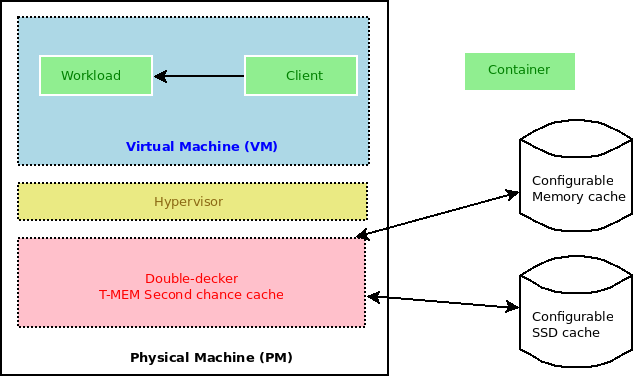
\includegraphics[width=0.9\textwidth]{images/correctness/exp_setup.png}
	  \caption{Experimental testbed for checking correctness}
	  \label{img:correctness_testbed}
	\end{figure}
	
      \subsubsection{Experimental configurations}	
	The set of configurations used for an analysis of memory management framework for a derivative environment 
	must be relevant, and easy to apply. The following configurations
fit this criteria, and have been used for the evaluation.

	  \begin{itemize}
	   \item \textbf{Memory Requirement:} Memory requirement of each container, the estimated total memory used by a container.
	   
	   \item \textbf{Container memory limit:} Size of memory allocated to a container at the Cgroup level (soft and hard limits). 
	   \item \textbf{Memory cache limit:} Size of memory (L1) cache assigned to a container. 
	   \item \textbf{SSD cache limit:} Size of SSD (L2) cache assigned to a container.
	   
	   \item \textbf{Workload:} Workload application that is running inside each of the container. 
	   \item \textbf{Number of containers:} Number of containers that are currently executing in the system.
	   \item \textbf{Number of VMs:} Number of virtual machines that are currently executing in the system.
	  \end{itemize}	  
	  
	  For the sake of simplicity in the evaluations of correctness of our setup. We have only considered a single container, single VM setup 
	  which makes use of synthetic workload to stress our system.
	
      \subsubsection{Metrics of interest}	
	The following are the metrics of interest that would help us establish the correctness of our implementation.
	  
	  \begin{itemize}
	   
	   \item \textbf{Container memory usage:} Guest memory usage of the container.
	   \item \textbf{Memory cache usage:} Memory cache used by the container.
	   \item \textbf{SSD cache usage:} SSD cache used by the container.
	   
	   \item \textbf{Demoted:} Objects moved from memory to SSD cache.
	   \item \textbf{Promoted:} Objects moved from SSD to memory cache.
	   
	  \end{itemize}	  
	  
	  The following metrics are collected both for memory and SSD cache
	  
	  \begin{itemize}
	   
	   \item \textbf{Puts:} Number of objects successfully put into this container cache.
	   \item \textbf{Gets:} Number of objects successfully got from this container cache.
	   \item \textbf{Flushes:} Number of objects flushed from this container cache.
	   \item \textbf{Evicts:} Number of objects evicted from this container cache.
	   
	  \end{itemize}
    
      \subsubsection{Workloads}
      
	This section presents the list of workloads that we have used as primary candidates to evaluate our empirical evaluations. All 
    workloads are chosen keeping in mind the memory intensive nature of the requirement.  
	
	These are the list of workloads we have used to establish issues and evaluate our framework.
	  
	  \myparagraph{Synthetic workload}
	    A self generated synthetic workload generated using \texttt{cat} command that outputs the 
	    content of a file onto \texttt{/dev/null}
	  
	  \myparagraph{MongoDB}
	    MongoDB \cite{Mongodb} is an open-source, document database designed for ease of development and scaling. Classified as a NoSQL 
    database program, MongoDB avoids the traditional table-based relational database structure in favor of JSON-like documents with dynamic 
    schema. It follows a memory hungry approach where it tries to use up most of system and it actually leaves it up to the OS's VMM to tell it 
    to release the memory.

	  \myparagraph{Redis}
	    Redis \cite{Redis} is a in-memory data structure store, used as database, cache and message broker. It is used to store a large 
    number of in-memory key-value pairs. Its in-memory nature makes it a prime candidate to use it as a workload in our empirical evaluations.
      
	  \myparagraph{MySQL}
	    MySQL \cite{mysql} is a database workload that uses anonymous pages to configure its own user-space data cache. 
	    
	  \myparagraph{Filebench}
	    Filebench \cite{filebench} is a synthetic workload used to generate workload patterns of different applications. In filebench we made
	    use of the webserver workload to simulate a webserver.
	  
      
	  \myparagraph{YCSB benchmark}
	    We use YCSB \cite{cooper2010benchmarking} (Yahoo Cloud Server Benchmark) project as the benchmark to generate the clients evaluate 
    to the performance of our real workloads i.e MongoDB, Redis and MySQL servers. The goal of YSCB is to develop performance comparisons of the new 
    generation of cloud data serving systems. It is a framework and common set of workloads for evaluating the performance of different 
    “key-value” stores.
  
    \subsection{Provisioning of caches at different levels based on application requirements}
    
      Previous results using \dd{}\cite{doubledecker} have shown that certain application requirements 
      (along with their configurations) could be satisfied better by provisioning on a cache of certain 
      performance guarantees. In the previous work\cite{doubledecker} it was shown how an application like 
      Mail-server could be better provisioned on the level-2 (SSD) cache, as its requirement involved 
      having a large WSS (working set size) with slow access rates. On contrary it also showed by cache sensitive 
      applications like the Web-server workload had to be provisioned onto the level-1 (memory) cache. 
      Now let's see if this setup of an exclusive two level cache provisioning schema would satisfy application
      specific need in all cases.
	
	\subsubsection{Inadequate exclusive two level cache provisioning}
	\label{sec:dd_hybrid_motivation}
	  
	  \myparagraph{Objective}
	    To demonstrate Inadequacy in exclusive two level cache provisioning under a tight memory-cache bound
	    scenario.  
	    
	  \myparagraph{Procedure}
	    Consider the following scenario to demonstrate the short comings of the existing exclusive two level cache
	    provisioning framework. Consider the case of a container running web-server workload
	    with a WSS to provisioned onto the hypervisor cache with  no-free memory to be further allocated 
	    at the guest VM and the hypervisor cache available is 0.5 GB at level-1 (Memory) and 1 GB at 
	    level-2 (SSD). Consider a Web-server workload where the desired application throughput is 7000 op/s.
	    
	  \begin{figure}
	    \centering
	    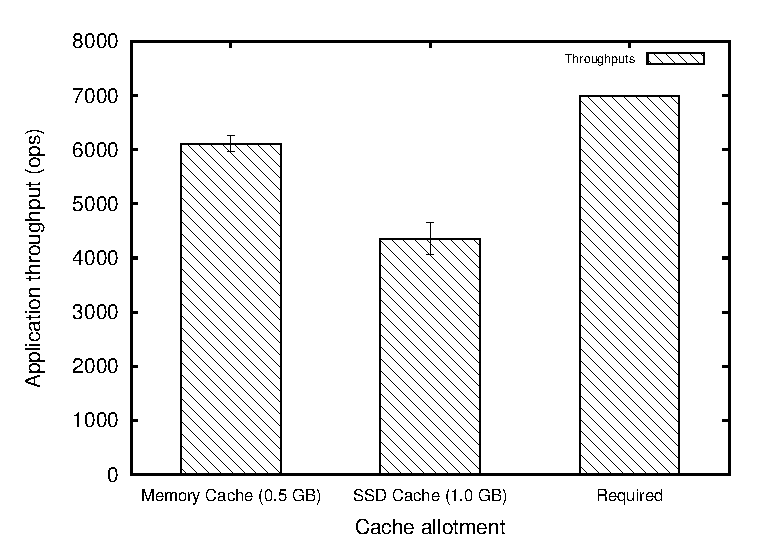
\includegraphics[scale=0.8]{images/dd_hybrid_motivation/throughput.eps}
	    \caption{Inadequate exclusive two level cache provisioning framework}
	    \label{plot:dd_hybrid_motivation}
	  \end{figure}
	  
	  \myparagraph{Inferences}
	    Using our existing double decker cache, we can at max provision at 6000 op/s using memory cache of 0.5 GB as 
	    shown in Fig~\ref{plot:dd_hybrid_motivation}. But say our requirement was beyond that at 7000 op/s. Is there a 
	    workaround to satisfy this requirement ? Could we come up with a better design to satisfy this configuration ?
	    
    
    \section{Cache partitioning framework support for anonymous memory applications} 
	
	\begin{figure}
	  \centering
	  \includegraphics[scale=0.8]{images/dd_decentrailze_motivation/throughput.eps}
	  \caption{Split of memory allocation ratios (In-VM:Cache) to affect application performance}
	  \label{plot:dd_decentrailze_motivation}
	\end{figure}
	
	\myparagraph{Objective}
	  To understand impact of memory provisioning at different levels of memory (In-VM or cache)
	  and how it impact application performance.
	
	\myparagraph{Procedure}
	  Application memory requirement is vastly classified into two types - \textit{anonymous and disk backed}.
	  Application that require disk backed memory pages can be satisfied be either provisioning them at the 
	  VM(guest) memory or at the hypervisor cache. We ran four different applications namely, Redis, \mongo{}
	  MySQL and Webserver and analyzed their impacts on memory provisioning.
	  
	\myparagraph{Observations}	  
	  This effect is seen in Fig~\ref{plot:dd_decentrailze_motivation}
	  where the memory requirement is split in ratios of in-VM:cache allocations. The plot shows how applications like
	  Web-server and \mongo{} which require disk backed pages can be satisfied either in-VM or at the hypervisor cache.
	  Kindly note that the application performance is nearly constant in all cases of both these applications as the 
	  in-VM memory and the hypervisor cache operate at similar speeds in this case, and had there been difference in
	  operational speeds, we would have observed degradation in application performance when moving from left to right 
	  in the plot.
	
	\myparagraph{Inference}
	  Now, if you look at applications like \redis{} and MySQL, their performance is highly affected while provisioning
	  them on cache, as they heavily depend on anonymous memory allocated to them (especially Redis). Hence such applications
	  need to be provisioned at the guest, however existing cache partitioning frameworks 
	  \cite{koller2015centaur, schopp2006resizing} can provision for disk backed workloads fail to address the needs of 
	  anonymous memory hungry workloads.
	    

  \section{Rethink of existing design}
    
    Keeping the above drawbacks in mind, we re-design the existing differentiated derivative cloud cache partitioning
    framework that \dd{} is and make it more of a memory management framework. There are two crucial ideas around which
    the design is centered around,
    
    \begin{enumerate}
      \item Decentralized memory management framework
      \item Hybrid two-level configurable caches
    \end{enumerate}
    
    \noindent These two components are discussed below.
  
    \begin{figure}
      \centering
      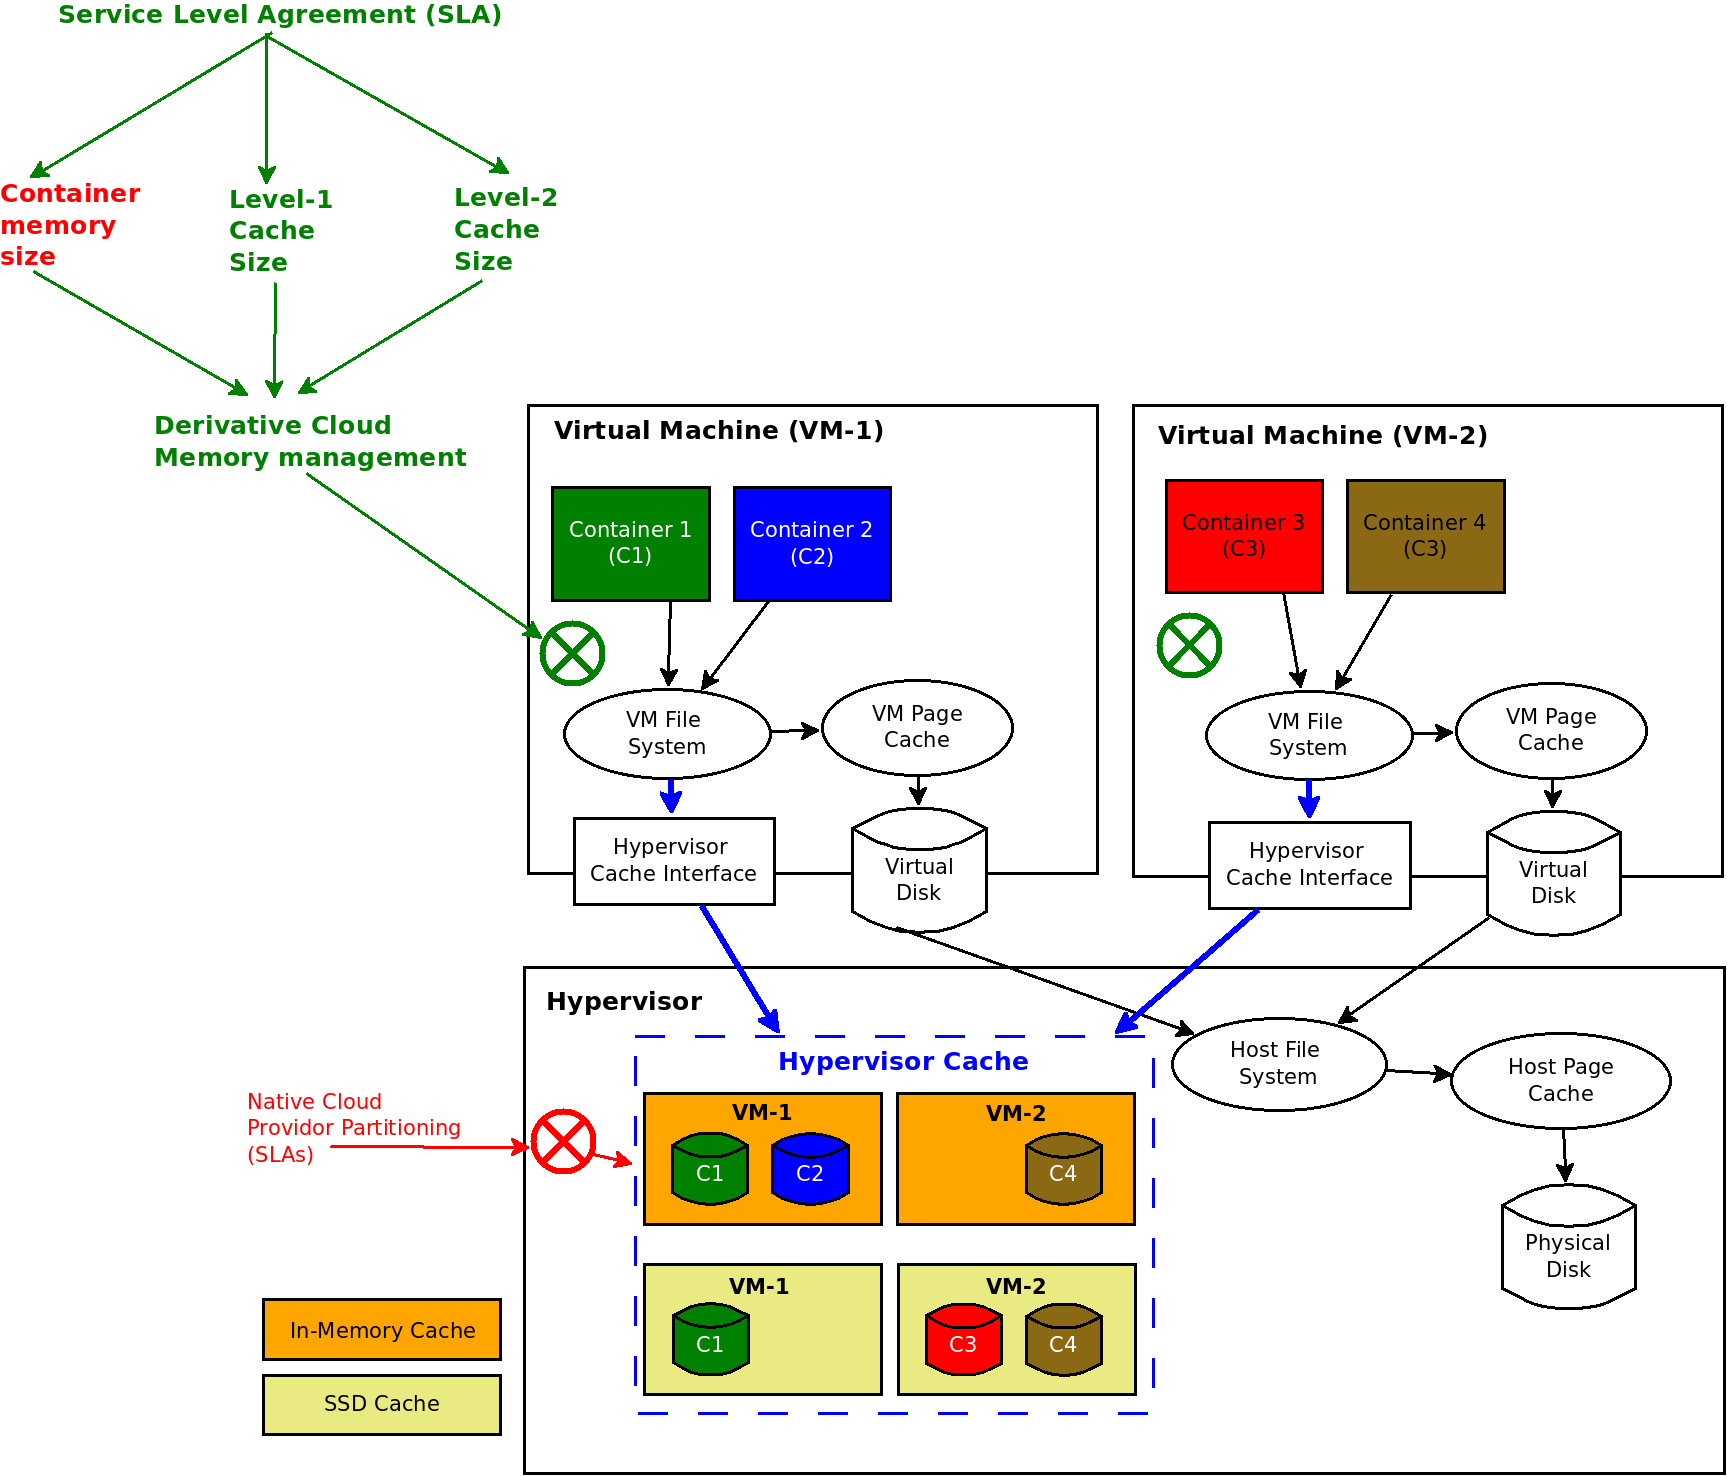
\includegraphics[scale=0.26]{/home/prashanth/Stage-2/Report/images/dd_design/architecture.png}
      \caption{Updated memory management framework}
      \label{plot:dd_architecture}
    \end{figure}
        
    \subsection{Decentralized memory management framework}
      Traditional caching frameworks and the earlier design of double decker centered around the idea 
      of a hypervisor managed cache with the hypervisor administrator (native cloud provider) as the single sole 
      administrator of the system.
      
      We now propose a decentralized memory management framework with two control centers 
      who roles each have been discussed below. Most of the decision making is moved onto the
      derivative cloud provider sitting inside the virtual machine.
	      
      \subsubsection{Native provider cache partitioning framework}
	The native provider is now, only responsible for partitioning the caches for each VM
	based on its native cloud provider SLA. The native provider need not worry about 
	provisioning each of the container.

      \subsubsection{Derivative provider memory management framework}	
	The derivative provider is now responsible for managing three levels of memory entities,
	
	\begin{enumerate}
	  \item Container memory size
	  \item In-memory or level-1 cache
	  \item SSD or level-2 cache
	\end{enumerate}
	
	The derivative provider maps each application SLA onto a combination of these three management
	knobs to achieve desired application level objectives. This helps even provisioning of applications
	that cannot be helped by cache partitioning schemas, that is that they are anonymous memory dependent.


    \subsection{Hybrid cache}
      The hybrid cache is an updated version of the previous cache where each VM/container can be configured
      with a in-memory and SSD cache simultaneously. But with two-levels of caches configured to each application
      we need an mechanism to move objects (pages) of one level to another and vice-versa.
      
      Every PUT operation into the cache tries to first add the new object into the memory cache if configured, 
      and if not it adds it to the SSD cache.
      
      \subsubsection{Movement of objects}	
	There are two levels of cache movements, and have thresholds which trigger this movement. The movement of
	objects are described below. The thresholds and the eviction batches are all configurable.
	
	The level-1 and level-2 caches have a higher threshold after which objects are either \textit{demoted} to the 
	lower level (in the case of level-1, if level-2 is configured) or is evicted from the cache. Similarly
	there is also an lower-threshold at level-1 and when the cache occupied at level-1 is below the lower threshold
	and objects are present at level-2, objects are \textit{promoted} to level-1 is triggered.
	
	The target execution entity (VM/container) for promotions or demotions are purely based on the entities that
	are exceeding their allocations the most (or) most under-utilizing their allocations. The order for selection
	is VM is selected first, followed by the container.
      
	
  \section{Implementation specifics of the hybrid cache}

    The hybrid cache implementation is built upon the existing implementation of the double decker cache as described in 
    Section~\ref{sec:double_decker_internals}. Changes have been made to this implementation to accommodate the hybrid setup.
    
    \begin{figure}
      \centering
      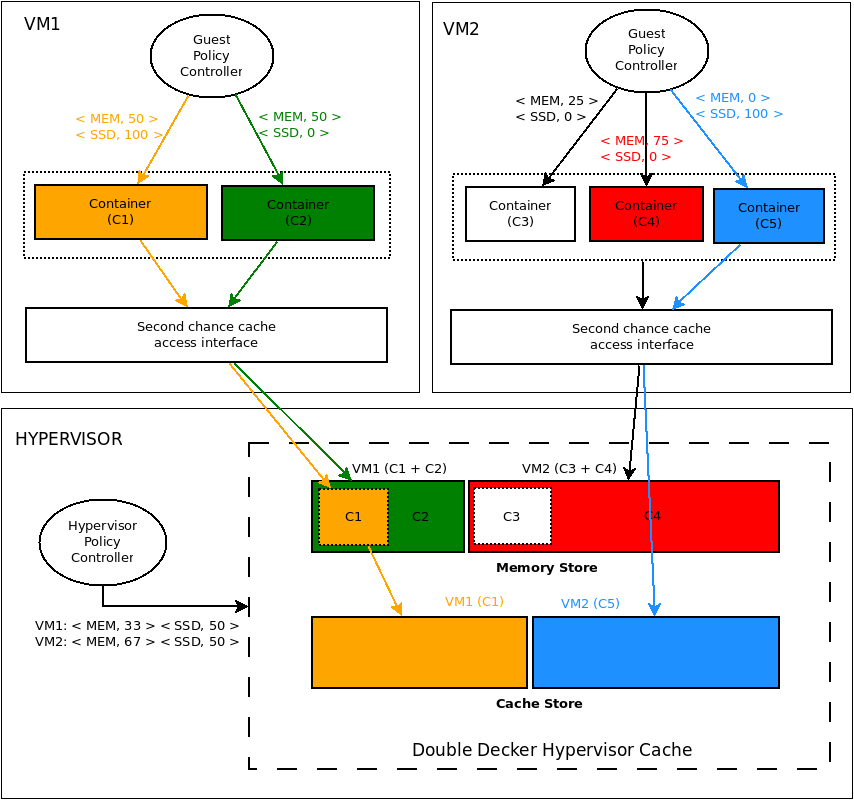
\includegraphics[width=0.75\textwidth]{/home/prashanth/Stage-2/Report/images/dd_design/implementation.png}
      \caption{\dd{} internals}
      \label{img:dd_internals}
    \end{figure}
  
      \subsubsection{Pool to accommodate both memory and SSD objects}
	The notion of pools as described in Section~\ref{sec:double_decker_internals} is carried over to the hybrid implementation.
	However, every pool for a particular container now contains a memory and SSD weight parameter. The VM also has a memory
	and SSD cache weight configuration parameter.
	
	The pool now stores both memory and SSD objects (as shown in Fig~\ref{img:dd_internals} using the same tree structure 
	that earlier stored a single type of object. The search mechanism is the same on the tree, but the tree node now either 
	points to a memory page or and SSD block based on the type of the node.  
	
	    
      \subsubsection{Asynchronous kernel threads for movement of objects}
	Two kernel threads were used to promote and demote objects between the two levels of cache. These kernel threads also
	performed eviction if movement of objects didn't clear up enough space. Asynchronous movement of threads required 
	proper synchronization and locking mechanisms to ensure consistency in data structure being manipulated. 
      
      \subsubsection{Multilevel stats}
	The stats that were earlier based on a single level, had to be changed to incorporate a multilevel stat. These 
	multilevel stats are developed to help provisioning of the three level knobs at the guest to satisfy application
	objectives.
  
  \section{Correctness of implementation}
  
      The experimental setup is just as described in Section~\ref{sec:dd_setup}.
      For establishing the correctness of our workload, we have considered a self 
      generated synthetic workload generated using \texttt{cat} command that 
      outputs the content of a file onto \texttt{/dev/null}. This workloads helps 
      us to validate the correctness of our implementation by predicting deterministic
      outputs.
  
    \subsection{Arithematic validation of stats}
    
      \myparagraph{Question}
	    To verify the correctness in accounting of stats while accessing cache at both levels.
	    
      \myparagraph{Procedure}
	We ran several experiments and computed the actual cache usage (memory and SSD) in our implementation. To an calculated 
	an estimated cache usage we used the formula given below. We used the same formula for both memory and SSD cache. 
	  \begin{equation}
	    EstimatedUsed = Puts + ObjectsMovedIn - (Gets + Flushes + ObjectsMovedOut)
	  \end{equation}
      
      \myparagraph{Observations}
	The values for \textit{EstimatedUsed} and \textit{ActualUsed} (present in out stat counter) matched in most cases.
	However, over long periods of run, with quite a large number of cache operations there was a marginal difference
	between the two (\textless 1\%).
	
      \myparagraph{Inference}
	Since the correctness of the actual value of cache used depend on the other stats that we have collected, and the 
	matching of \textit{EstimatedUsed} and \textit{ActualUsed} would only mean that all the stats collected are right.
    
    \subsection{Movement of objects between both levels of cache}
	
	To verify the correctness of our implementation empirically, we have taken our synthetic workload described in 
	above and ran a couple of simple experiments to demonstrate the expected 
	behavior of our cache to support cache operations like puts, gets, promotions and demotions.  
	
	\subsubsection{Memory to SSD cache}

	  \myparagraph{Question}
	    To verify the correctness in accounting of stats while accessing cache and moving objects from memory (L1) to SSD (L2) cache.
	    
	  \myparagraph{Procedure}
	      We start of the experiment with powering on the VM, followed by the container. We assigned complete memory and SSD cache 
	    at the double-decker back-end to support the container. The container had a \textbf{memory requirement of 2078 MB}, 2048 MB workload
	    requirement and 30 MB container requirement (container requirement was obtained by running the same experiment while having
	    a nearly 0 MB workload. The container was allocated with 2048 MB (512 MB of container memory + 512 MB of memory cache 
	    + 1024 MB of SSD cache). Now, the workload performed a sequential read of its workload (i.e 2048 MB) once.
	    Table~\ref{table:correctness_memtossd} shows the list of approx. estimated values (which are based on our 
	    implementation) and observed values for the metrics at the cache at the end of the experiment. 
	    
	    \vspace*{1em}	
	      \begin{table}
		\begin{center}
		  \begin{tabular}{ r | p{4cm} | p{4cm} }	      	    
			Metric & Approx. estimated Value & Observed Value \\ 
		    \hline
		    \hline
		    Puts (MB) & 2078 & 2080 \\
		    \hline
		    Gets (MB) & 0 & 1 \\
		    \hline
		    Container memory usage (MB) & 512 & 509 \\  
		    \hline
		    Memory cache usage (MB) & 504 & 503 \\
		    \hline 
		    SSD cache usage (MB) & 1008 & 1000 \\
		    \hline
		    Evicts (MB) & 54  & 64 \\
		    \hline
		    Flushes (MB) & 0  & 0 \\
		    \hline
		    Cumulative usage (MB) & 2078 & 2076 \\
		    \hline
		    Demotions (MB) & 1062 & 1064 \\
		    \hline
		    
		  \end{tabular}
		\caption{Comparison between expected and actual values}
		\label{table:correctness_memtossd}
		\end{center}	  
	      \end{table}
	    \vspace*{1em}
	    
	  \myparagraph{Observations}
	  The following are the observations,	  
	    \begin{enumerate}
	     \item There is a small number of gets, probably occurring due to pages used by other container applications.
	     \item Puts in the cache, is marginally (\textless2 MB) greater than expected value, and this deviation is due to the small number 
	     of Gets which are occurring.
	     \item The memory cache usage, is exactly as expected. However, SSD cache usage is slightly lesser than the expected value, 
	     but however the deviation seems to be an acceptable value.
	     \item The demotions (movement from memory to SSD) and cumulative usage values are nearly the same with a subtle deviation 
	     (\textless2 MB) which is an acceptable value.
	    \end{enumerate}

	  
	  \myparagraph{Inference}
	    The accounting stats, are nearly as expected. This verifies the correctness of most of the stats of our implementation (except promotions).
	    
	
	\subsubsection{SSD to memory cache}
	  
	  \myparagraph{Question}
	    To verify the correctness in accounting of stats while moving objects from SSD (L2) to memory (L1) cache.
	    
	  \myparagraph{Procedure}
	      We start of the experiment with powering on the VM, followed by the container. We assigned complete memory and SSD cache 
	    at the double-decker back-end to support the container. The container had a \textbf{memory requirement of 2078 MB}, 2048 MB workload
	    requirement and 30 MB container requirement (container requirement was obtained by running the same experiment while having
	    a nearly 0 MB workload. The container was allocated with 2560 MB (512 MB of container memory + 2048 MB of SSD cache).
	    The workload performed a sequential read of its workload (i.e 2048 MB) once, this lead to using up of nearly 1566 MB of SSD cache.
	    
	    Now, we changed the memory cache size to 256 MB while performing basic operations at the container which triggered the promotion 
	    (movement of objects from SSD to memory) of the objects to the memory cache. The promotion triggers all objects until the memory 
	    cache reaches a threshold usage - 192 MB in our case, as this threshold is calculated as,
	    
	    \begin{equation}
	      MemoryCacheLowerThreshold (192 MB) = MemoryLimit (256 MB) - LimitSize (64 MB)
	    \end{equation}
	    
	    Hence we would expect 192 MB worth of objects be promoted from SSD to memory cache in an ideal case.
	    
	    
	  \myparagraph{Observation}
	    Using our stats, it was observed that the estimated promotion and the actual promotion of objects were of an exact match with 
	    the number being 192 MB.
	    
	  \myparagraph{Inference}
	    This verifies the correctness in the accounting stats in movement of objects from SSD to memory cache. Hence movement 
	    of objects from both memory to SSD and vice-versa have been verified empirically.
  
  
  
  \section{Evaluation of Double Decker}
    Now, that we have established correctness of our implementation, we had put it to test its effectiveness in 
    tackling in previously mentioned drawbacks. The experimental setup is configured as described in Section~\ref{sec:dd_setup}
    
    %\subsection{Performance comparion with old implementation}
  
    \subsection{Hybrid cache provisioning}
    
       \myparagraph{Objective}
	To demonstrate the effectiveness of the hybrid cache partitioning design to achieve application objectives
	better than an exclusive two level cache partitioning.
	
      \myparagraph{Setup}
	Setup used is as described in Section~\ref{sec:dd_setup}.
	
      \myparagraph{Procedure}
	Configuration of the experiment is given at Section~\ref{sec:dd_hybrid_motivation}, the WSS of the workload is
	1 GB. We fix the total cache allocation (Memory + SSD) at 1 GB.	To demonstrate the effectiveness of our 
	implementation we vary cache allocation ratios from all cache allocations at level-1 to all at level-2 and 
	see how this affects application performance.
	
	\begin{figure}
	  \centering
	  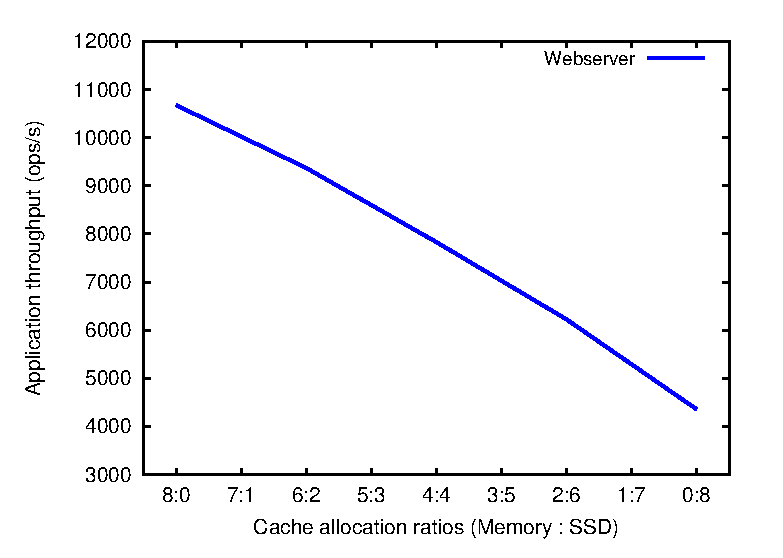
\includegraphics[scale=1]{images/dd_hybrid_eval/throughput.eps}
	  \caption{Varying of cache allocation ratios while achieving application level throughputs}
	  \label{plot:dd_sdc_results}
	\end{figure}
	
      \myparagraph{Observation}
	The application throughput increase as moving the cache partitioned from memory onto the SSD as expected.
	To satisfy an application objective of 7000 ops/sec as discussed in Section~\ref{sec:dd_hybrid_motivation}, 
	cache would have to partitioned at about 4:4 ratio in this case, which refers to 512MB of memory and SSD 
	cache each.
	
      \myparagraph{Inference}
	An hybrid implementation is more effective at satisfying SLA objectives for cases where an two level exclusive
	caching setup fails.
	
    \subsection{Effectiveness of our decentralized memory management framework}
      
      \myparagraph{Objective}
	To demonstrate the effectiveness of the cooperative memory management framework in achieving desired application 
	objectives which traditional cache partitioning frameworks cannot.
	
      \myparagraph{Setup}
	VM hosted 4 application containers and executed the MongoDB, Redis, MySQL data stores and
	the Filebench Web-server workload. The data stores acted as backends for YCSB clients. The VM 
	was provisioned with 6GB memory and 8 CPUs (2 CPUs pinned to each application container). 
	The hypervisor cache was provisioned to 2GB.
	
      \myparagraph{Procedure}
	To approximate the best cache partitioning framework, we iterated through a series of possible 
	configurations and have reported the best cache partitioning schema. 
	
	Consider the case where the application throughput requirements of the different applications running
	are as described in Table~\ref{table:desired_app_throughputs}
	
	    \begin{table}
		\begin{center}
		  \begin{tabular}{ l | l | l | l | l }	      	    
			Workload & MongoDB & MySQL & Redis & Webserver \\ 
		    \hline
			Required throughput & 15 ops/sec & 100 ops/sec & 5000 ops/sec & 300 ops/sec \\		   
		  \end{tabular}
		\caption{Application SLA requirements}
		\label{table:desired_app_throughputs}
		\end{center}	  
	      \end{table}
	  
	The best configuration was the one met individual application SLAs and yielded the maximum application 
	throughputs.	
		
	We have taken frameworks as described below and compare them against one another in achieving application level objectives.
	  \begin{enumerate}
	    \item \textbf{Best cache partitioning - No memory allocations:} Double decker configurations with best cache partitioning
	    and no memory allocation.
	    \item \textbf{Best cache partitioning - Uniform memory allocations:} Double decker configurations with best cache partitioning
	    and uniform memory allocation.
	    \item \textbf{Best cache partitioning - Best memory allocations:} Double decker configurations with best cache partitioning
	    and best memory allocations given based on requirement stats obtained from memory \cg{}.
	  \end{enumerate}
    
      \myparagraph{Observations}
	As Observed in Fig~\ref{plot:dd_sdc_results}, our decentralized memory management framework depicted by 
	\textit{Best cache partitioning - Best memory allocations} is the only able to achieve application level 
	objectives. This prominently true in cases of Redis and MySQL which are anonymous memory hungry workloads
	as provisioning in the cache isn't going to help them achieving application throughputs.
	
	\begin{figure}
	  \centering
	  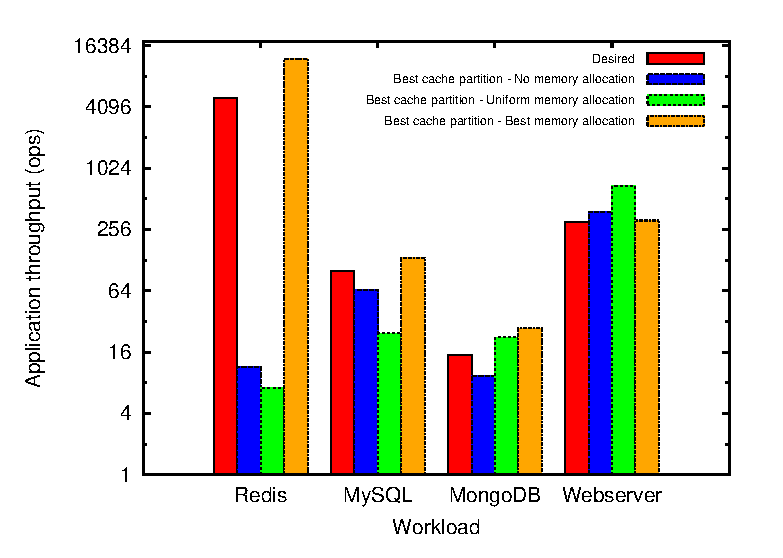
\includegraphics[scale=1]{images/dd_sdc_plot/sdc_dd.eps}
	  \caption{Achieved application performance using different types of frameworks}
	  \label{plot:dd_sdc_results}
	\end{figure}
	
      
      \myparagraph{Inference}
	Two-level provisioning capability of \dd{} enables holistic memory configurations 
	which can account for application characteristics and requirements, and yield improved
	application-level and system-wide performance. For workload provisioning in an adaptive manner, 
	\dd{} can employ well known techniques like MRC \cite{zhao2009dynamic, zhou2004dynamic}, 
	WSS estimation \cite{zhao2011low}, SHARDS \cite{waldspurger2015efficient} etc.. Note that, the estimation
	should be done from within the VM which allows the guest
	OS memory manager to provision memory resources at the
	two levels. Centralized nesting agnostic hypervisor cache
	management techniques cannot explore such provisioning
	configurations
      
      
      
    